\section{Language Performance Trade-offs}
\label{sec:language-performance}

This section compares the four \emph{implementations} on the shared workload.
It reports what was measured; it does not generalise to the languages
themselves (see \cref{sec:limitations}).

\subsection{Executive radar}
\label{sec:radar}

\begin{figure}[htbp]
    \centering
    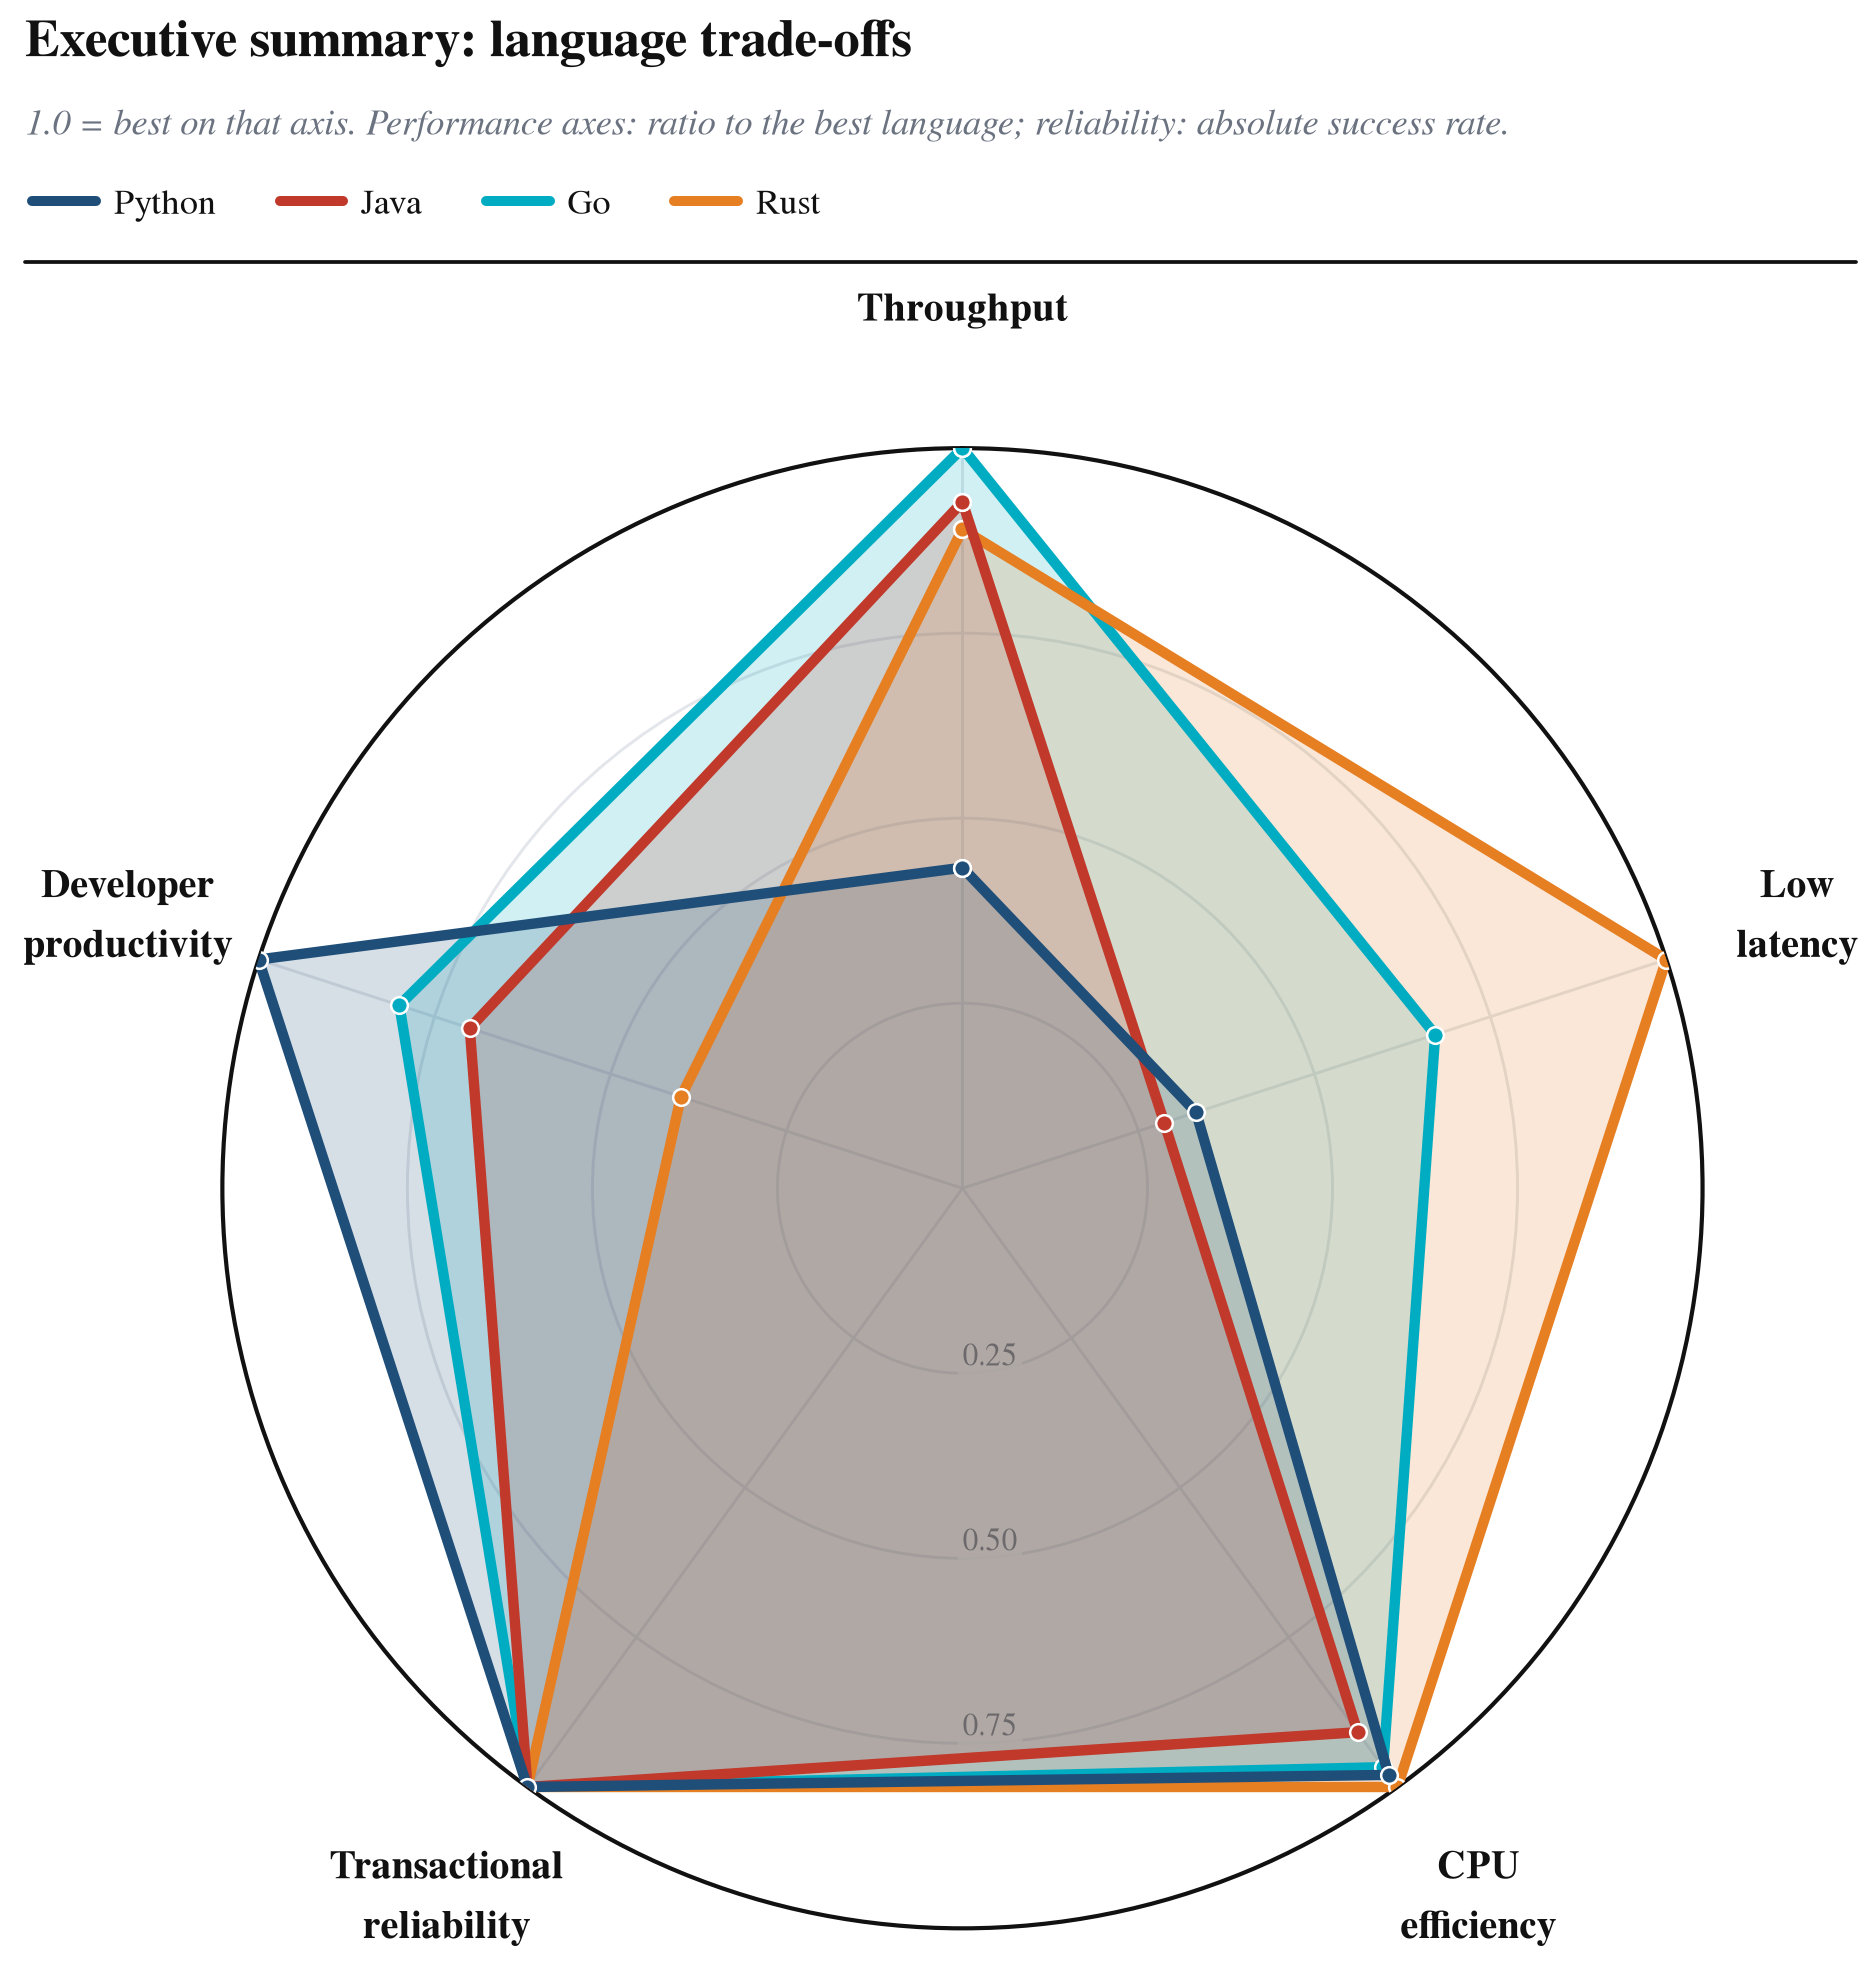
\includegraphics[width=0.60\textwidth]{radar/executive_radar.png}
    \caption{Five-axis executive summary (generated by
    \texttt{src/visualizations/main.py} from
    \texttt{benchmarks\_results/}). Throughput, low latency and CPU
    utilisation are ratios to the best implementation on tests run by all
    four languages; reliability is an absolute rate; ``developer
    productivity'' is a \textbf{qualitative} team score, although the axis
    label in the image does not yet say so (\cref{sec:radar}).}
    \label{fig:radar}
\end{figure}

The radar of \cref{fig:radar} summarises five axes. Four are computed from
the CSVs:

\begin{itemize}
    \item \textbf{Throughput, low latency, CPU efficiency} --- ratios to the
    best measured implementation on tests run by \emph{all four} languages,
    so no axis is biased by a partial run;
    \item \textbf{Transactional reliability} --- an absolute success rate,
    $1 - (\text{lost} + \text{duplicated}) / \text{total books}$, averaged
    over the recovery scenarios. It is deliberately \emph{not} rescaled to
    the best language: an implementation that loses books must never be
    stretched to 1.0.
\end{itemize}

The fifth axis, \textbf{developer productivity}, is a \emph{qualitative
score} assigned by the team (Python 1.0, Go 0.8, Java 0.7, Rust 0.4) from
the effort observed while porting the pipeline: lines of boilerplate,
error-handling ceremony, iteration speed and tooling friction. It is not
measured by any benchmark and no conclusion in \cref{sec:conclusions} rests
on it; this paragraph is the authoritative reading of that axis, whose
rendered label does not yet say ``qualitative'' (\cref{sec:future}).
Memory is intentionally absent from the radar: RSS deltas are too
noisy to summarise in one number; they are shown in full in
\cref{fig:scalability-memory}.

\paragraph{Scores in the current snapshot.}
Throughput: Go 1.00, Rust 0.88, Java 0.73, Python 0.72. Low latency: Rust
1.00, Go 0.74, Python 0.35, Java 0.21. CPU axis: Go 1.00, Rust 0.98, Java
0.94, Python 0.94. Reliability: 1.00 for all four. Three caveats bound this
summary:

\begin{itemize}
    \item The throughput axis is the geometric mean of the three datalake
    write rates and the download rate. The rendered figure takes only the
    fifth of the five download rounds instead of their mean (the per-round
    rows are in \texttt{throughput.csv}). With the five-round mean the scores
    are Go 1.00, Rust 0.82, Python 0.68 and Java 0.68: Go and Rust keep their
    order, Python and Java become indistinguishable.
    \item The CPU axis scores \emph{lower} mean CPU utilisation during the
    index builds as better, so a client that waits on \texttt{mongod} scores
    well. It measures utilisation, not efficiency; with every harness pinned
    to one core the four raw values span only 85.4--90.9\%, and no conclusion
    is drawn from it.
    \item The reliability axis is 1.0 by construction of the resume check
    (\cref{sec:datalake-recovery}) and cannot discriminate between the
    implementations.
\end{itemize}

\subsection{Throughput and latency overview}
\label{sec:throughput-latency}

\begin{figure}[htbp]
    \centering
    \begin{minipage}[t]{0.48\textwidth}
        \centering
        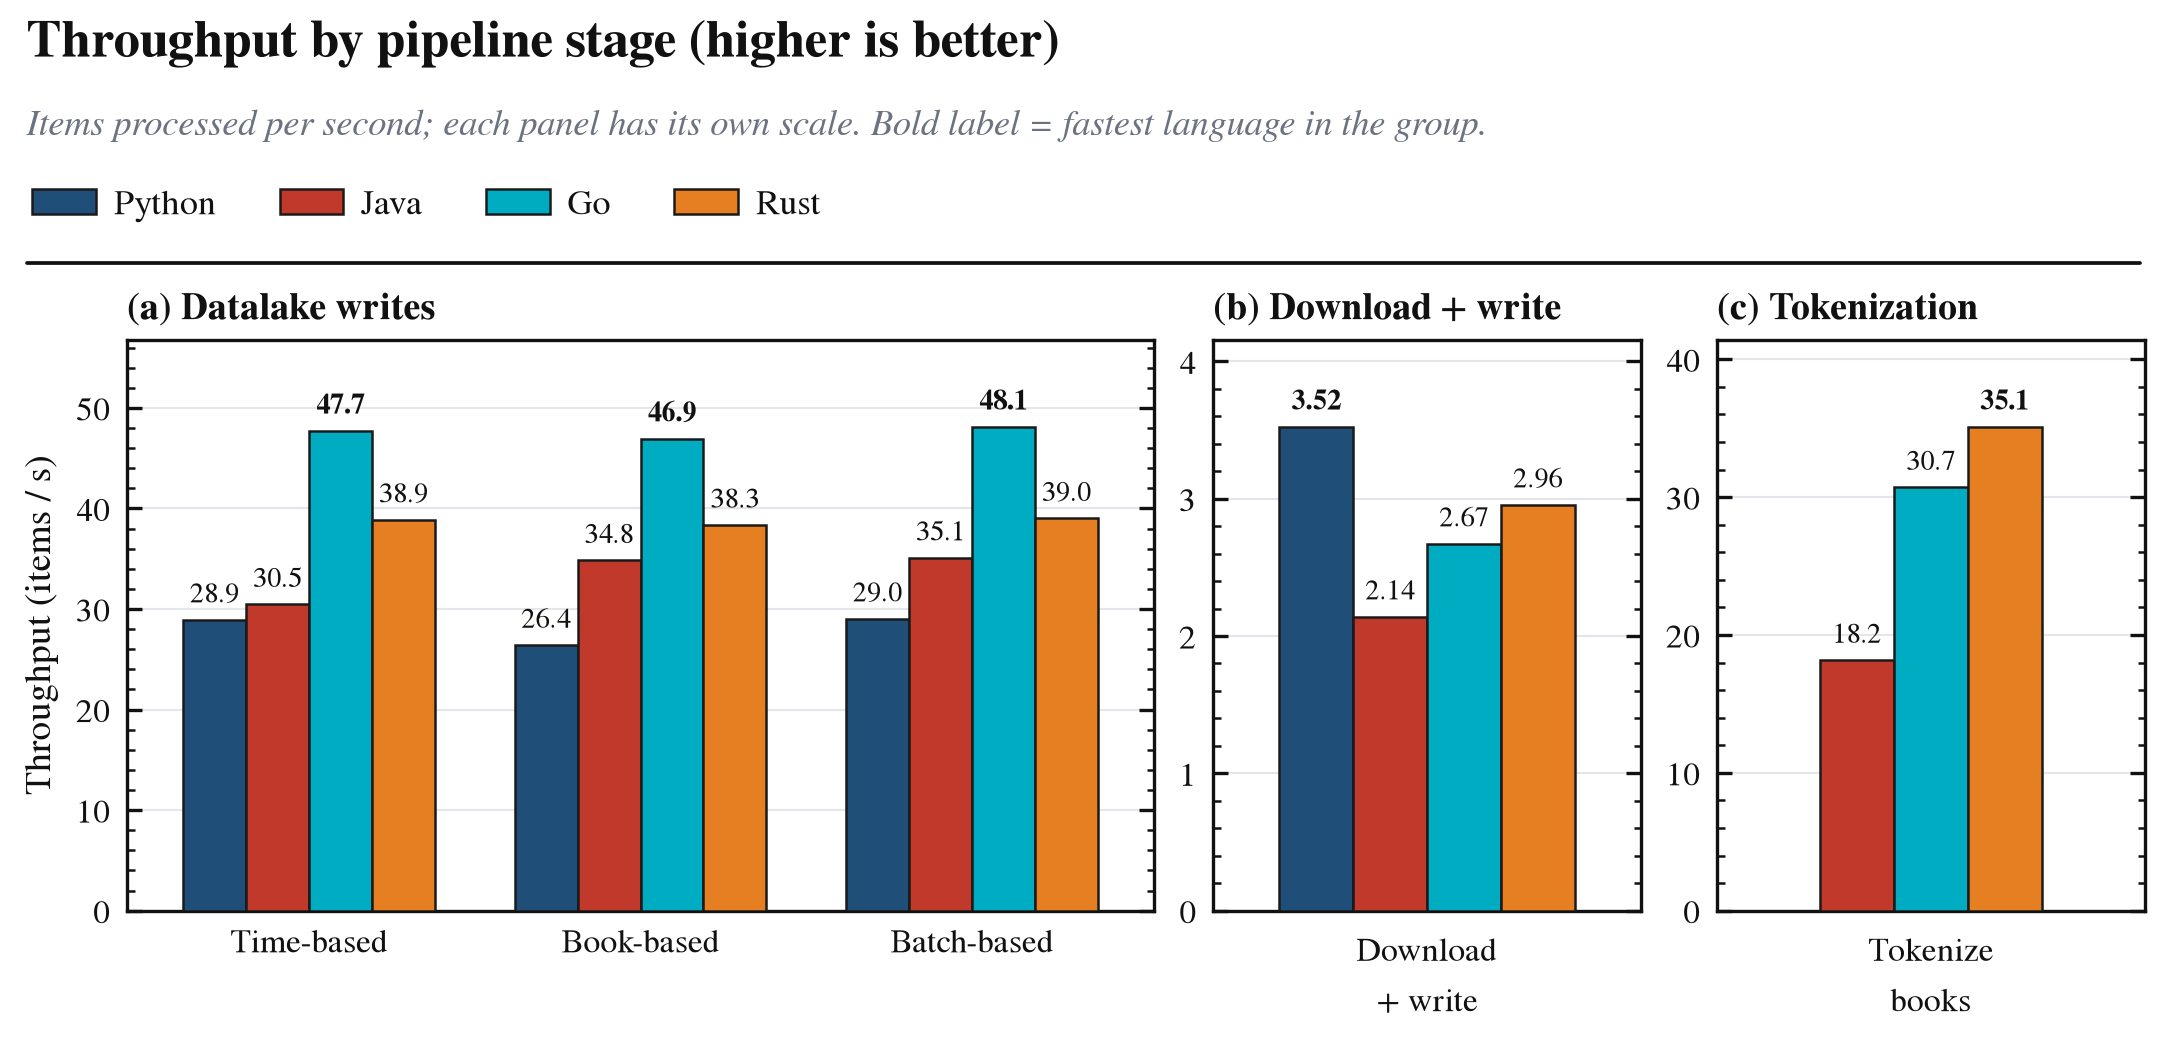
\includegraphics[width=0.95\textwidth]{throughput/throughput.png}
        \caption{Throughput per pipeline stage: (a) datalake writes, one
        timed run of 100 books per layout; (b) download + write, 10 books
        per round, showing the fifth of five rounds (five-round means in
        \cref{tab:download}); (c) tokenisation of the corpus (not recorded
        by the Python harness).}
        \label{fig:throughput}
    \end{minipage}\hfill
    \begin{minipage}[t]{0.48\textwidth}
        \centering
        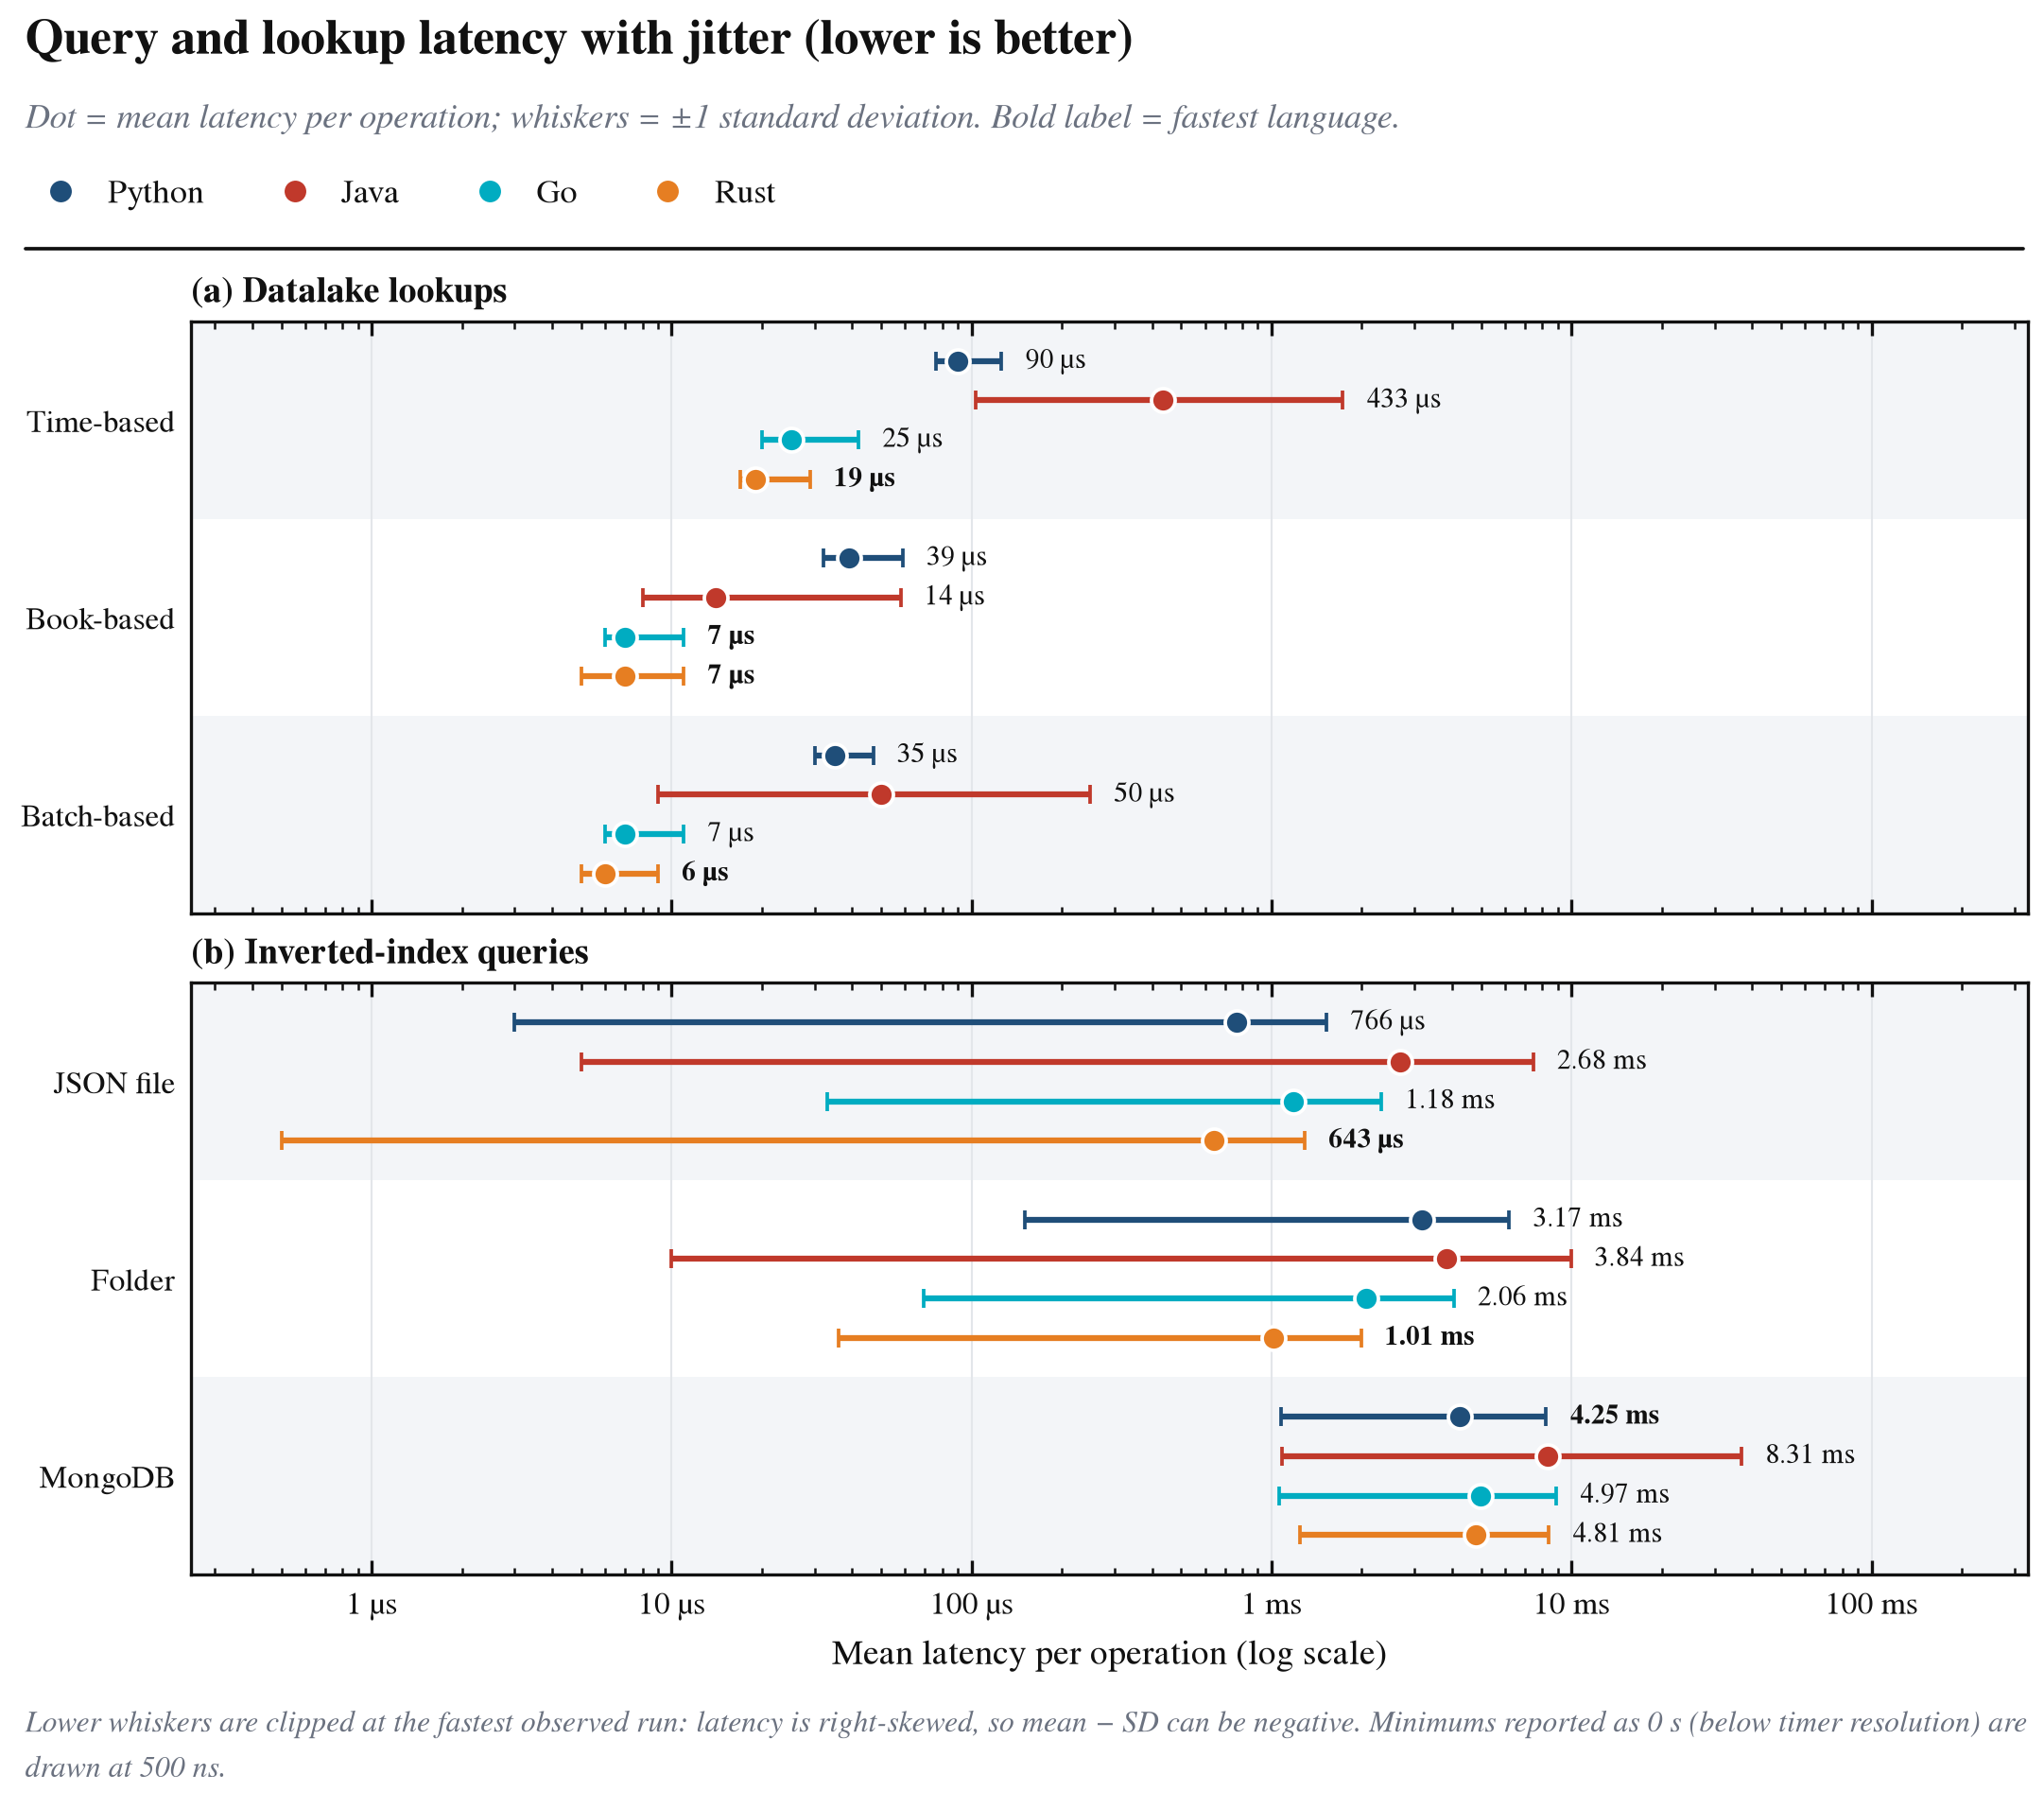
\includegraphics[width=0.95\textwidth]{latency/latency.png}
        \caption{Lookup latency per datalake layout (100 samples) and query
        latency per index structure (150 samples on the 10{,}000-book
        index). Dot = mean; whiskers = $\pm 1$ SD, clipped at the
        minimum.}
        \label{fig:latency}
    \end{minipage}
\end{figure}

\Cref{fig:throughput,fig:latency} show the two extremes of the workload.
They come from the same tournament run, so their relative ordering is
meaningful; the absolute values are specific to the host of
\cref{tab:host}, and the raw rows sit next to them in
\texttt{benchmarks\_\allowbreak results/}.

The reading rule for this whole report: differences between the four
implementations describe \emph{these implementations, on this corpus, under
this protocol}. Where an explanation requires a language-level cause (JIT
behaviour, allocator strategy, runtime overhead), it is stated as a
hypothesis and flagged as such, not as a measured fact.

\subsection{Effect of the corrective changes}
\label{sec:refactor-effect}

Between the snapshot discussed in the previous version of this report
(results commit \texttt{28d4c3f}, run of 25 October, code \texttt{b104a9a})
and the current one (results commit \texttt{9e53348}, run of 28 October,
code \texttt{0482a5e}), five changes were made to the ports and the harness.
None of them alters what is computed (the equivalence digest of
\cref{sec:equivalence} is unchanged) or introduces concurrency.
\Cref{tab:refactor-effect} pairs each change with the metric it should
move.

\begin{table}[htbp]
    \centering
    \small
    \caption{Previous $\to$ current value of the metrics each corrective
    change targets (one tournament run per snapshot; raw rows in
    \texttt{benchmarks\_results/} at \texttt{28d4c3f} and \texttt{9e53348}).}
    \label{tab:refactor-effect}
    \begin{tabularx}{\textwidth}{@{}Xrrrr@{}}
        \toprule
        Metric & Python & Go & Rust & Java \\
        \midrule
        \multicolumn{5}{@{}l}{\emph{Durable writes (temporary file, fsync, rename) in every port}} \\
        Datalake write, items/s (mean of 3 layouts) & 29.2$\to$28.1 & 68.0$\to$47.6 & 79.1$\to$38.7 & 64.6$\to$33.5 \\
        \multicolumn{5}{@{}l}{\emph{Pooled HTTP connection; five interleaved download rounds}} \\
        Download + write, items/s (5-round mean) & 1.48$\to$3.24 & 3.32$\to$3.12 & 1.32$\to$2.60 & 2.87$\to$1.88 \\
        \multicolumn{5}{@{}l}{\emph{Rust MongoDB update sent as one bulk write per book}} \\
        MongoDB update, base 25, ms & 134$\to$128 & 124$\to$113 & 474$\to$122 & 130$\to$145 \\
        MongoDB update, base 1{,}000, ms & 381$\to$397 & 293$\to$299 & 643$\to$286 & 294$\to$305 \\
        \multicolumn{5}{@{}l}{\emph{Collection dropped, not emptied, before every build}} \\
        MongoDB \texttt{storageSize}, MiB & 557.1$\to$29.6 & 558.9$\to$5.4 & 324.6$\to$16.1 & 38.2$\to$13.1 \\
        \multicolumn{5}{@{}l}{\emph{Every harness pinned to one logical core}} \\
        Build, 10{,}000 books, JSON, s & 167.1$\to$170.9 & 66.0$\to$71.4 & 196.4$\to$208.1 & 947.0$\to$1154.4 \\
        Build, 10{,}000 books, folder, s & 234.7$\to$215.3 & 69.9$\to$78.4 & 202.7$\to$198.1 & 955.2$\to$1130.0 \\
        Build, 10{,}000 books, MongoDB, s & 220.7$\to$181.5 & 76.6$\to$83.8 & 206.6$\to$200.7 & 929.1$\to$1185.1 \\
        \bottomrule
    \end{tabularx}
\end{table}

\paragraph{Durability, not language, explained most of the earlier write gap.}
In the previous snapshot only the Python baseline wrote datalake files
through a temporary file, \texttt{fsync} and rename; the ports used plain
writes, and the write-throughput spread was $3.0\times$ (27.3--82.8
items/s). With the same protocol in all four, the ports lost 30\% (Go), 51\%
(Rust) and 48\% (Java) of their rate, while Python, whose write path did not
change, moved by $-4\%$; the spread fell to $1.8\times$ (26.4--48.1
items/s). Python thus acts as an internal control: the host-level
differences between the two runs moved its unchanged write path by a few
per cent only, so the ports' drops are attributable to the added
synchronisation. Client CPU utilisation during the writes fell in every port
(Go 35--38\% $\to$ 17--18\%, Rust 17--19\% $\to$ 10--13\%, Java 36--70\% $\to$ 27--37\%), as
expected when a phase becomes storage-bound (\cref{sec:datalake-throughput}).

\paragraph{Rust's MongoDB update cost was a protocol artefact.}
The Rust port previously issued one \texttt{update\_one} round trip per
distinct term; it now sends the same upserts as one unordered bulk write,
like the other three. Its single-book update at base 25 fell from 474 to
122~ms ($3.9\times$) and now lies within the 113--145~ms band of the other
ports. The previous flat Rust curve ($1.36\times$ from base 25 to 1{,}000)
came from a large constant round-trip cost hiding the growth; with the bulk
write Rust grows $2.34\times$, in line with the others
(\cref{sec:index-updates}).

\paragraph{Collection reuse inflated the MongoDB footprint.}
Dropping the collection before each build reduced the reported
\texttt{storageSize} from 38.2--558.9~MiB to 5.4--29.6~MiB. The remaining
$5.5\times$ spread for identical logical content shows that the figure is
still not a reliable footprint measure (\cref{sec:index-structures}).

\paragraph{Pinning penalised the runtimes that parallelise their own housekeeping.}
Under the single-core budget the 10{,}000-book builds became 8--12\% slower
in Go and 18--28\% slower in Java, whereas Python and Rust, whose timed code
runs no background runtime threads, changed by $-18$ to $+6\%$ without a
consistent direction. Go's concurrent garbage collector and the JVM's
collector and JIT compiler threads previously ran on other cores and now
share the measured one; in addition, with one processor reported, HotSpot's
ergonomics select the Serial collector instead of G1, so the current Java
series runs under a different collector than the previous one. This
attribution is a hypothesis: no GC log was recorded. We do not attribute the
Python and Rust movements.

\paragraph{What the comparison cannot separate.}
Both snapshots are single runs, and more than the five changes differ
between them: the memory visible to the WSL2 virtual machine (7.66 $\to$
9.71~GiB), the toolchain patch versions (Go 1.27.1 $\to$ 1.27.2, Rust 1.99.0
$\to$ 1.99.1, OpenJDK 21.0.12.1 $\to$ 21.0.13) and the MongoDB server record
(\texttt{mongo:7} in Docker now; the previous record could not identify the
server). Only the effects with a direct mechanism (synchronisation, bulk
write, collection drop) are attributed above; the rest of this report
interprets the current snapshot on its own.
